\section{Architecture du Projet}
Pour notre Projet, nous avons créé plusieurs package différents afin d'avoir un espace de travail ordonné et rigoureux.
Ainsi nous avons un package \textbf{build} contenant toute les classes après compilation, un package \textbf{doc} contenant toute la javadoc compilé, un package \textbf{lib} contenant la librairie afin d'exécuter correctement les tests, un package \textbf{ressource} qui contient les package CSV, img et RLE contenant respectivement les fichiers au format .csv, .png et .rle et enfin nous avons le package \textbf{src} qui contient tout notre code. 
\begin{figure}[htp]
\centering
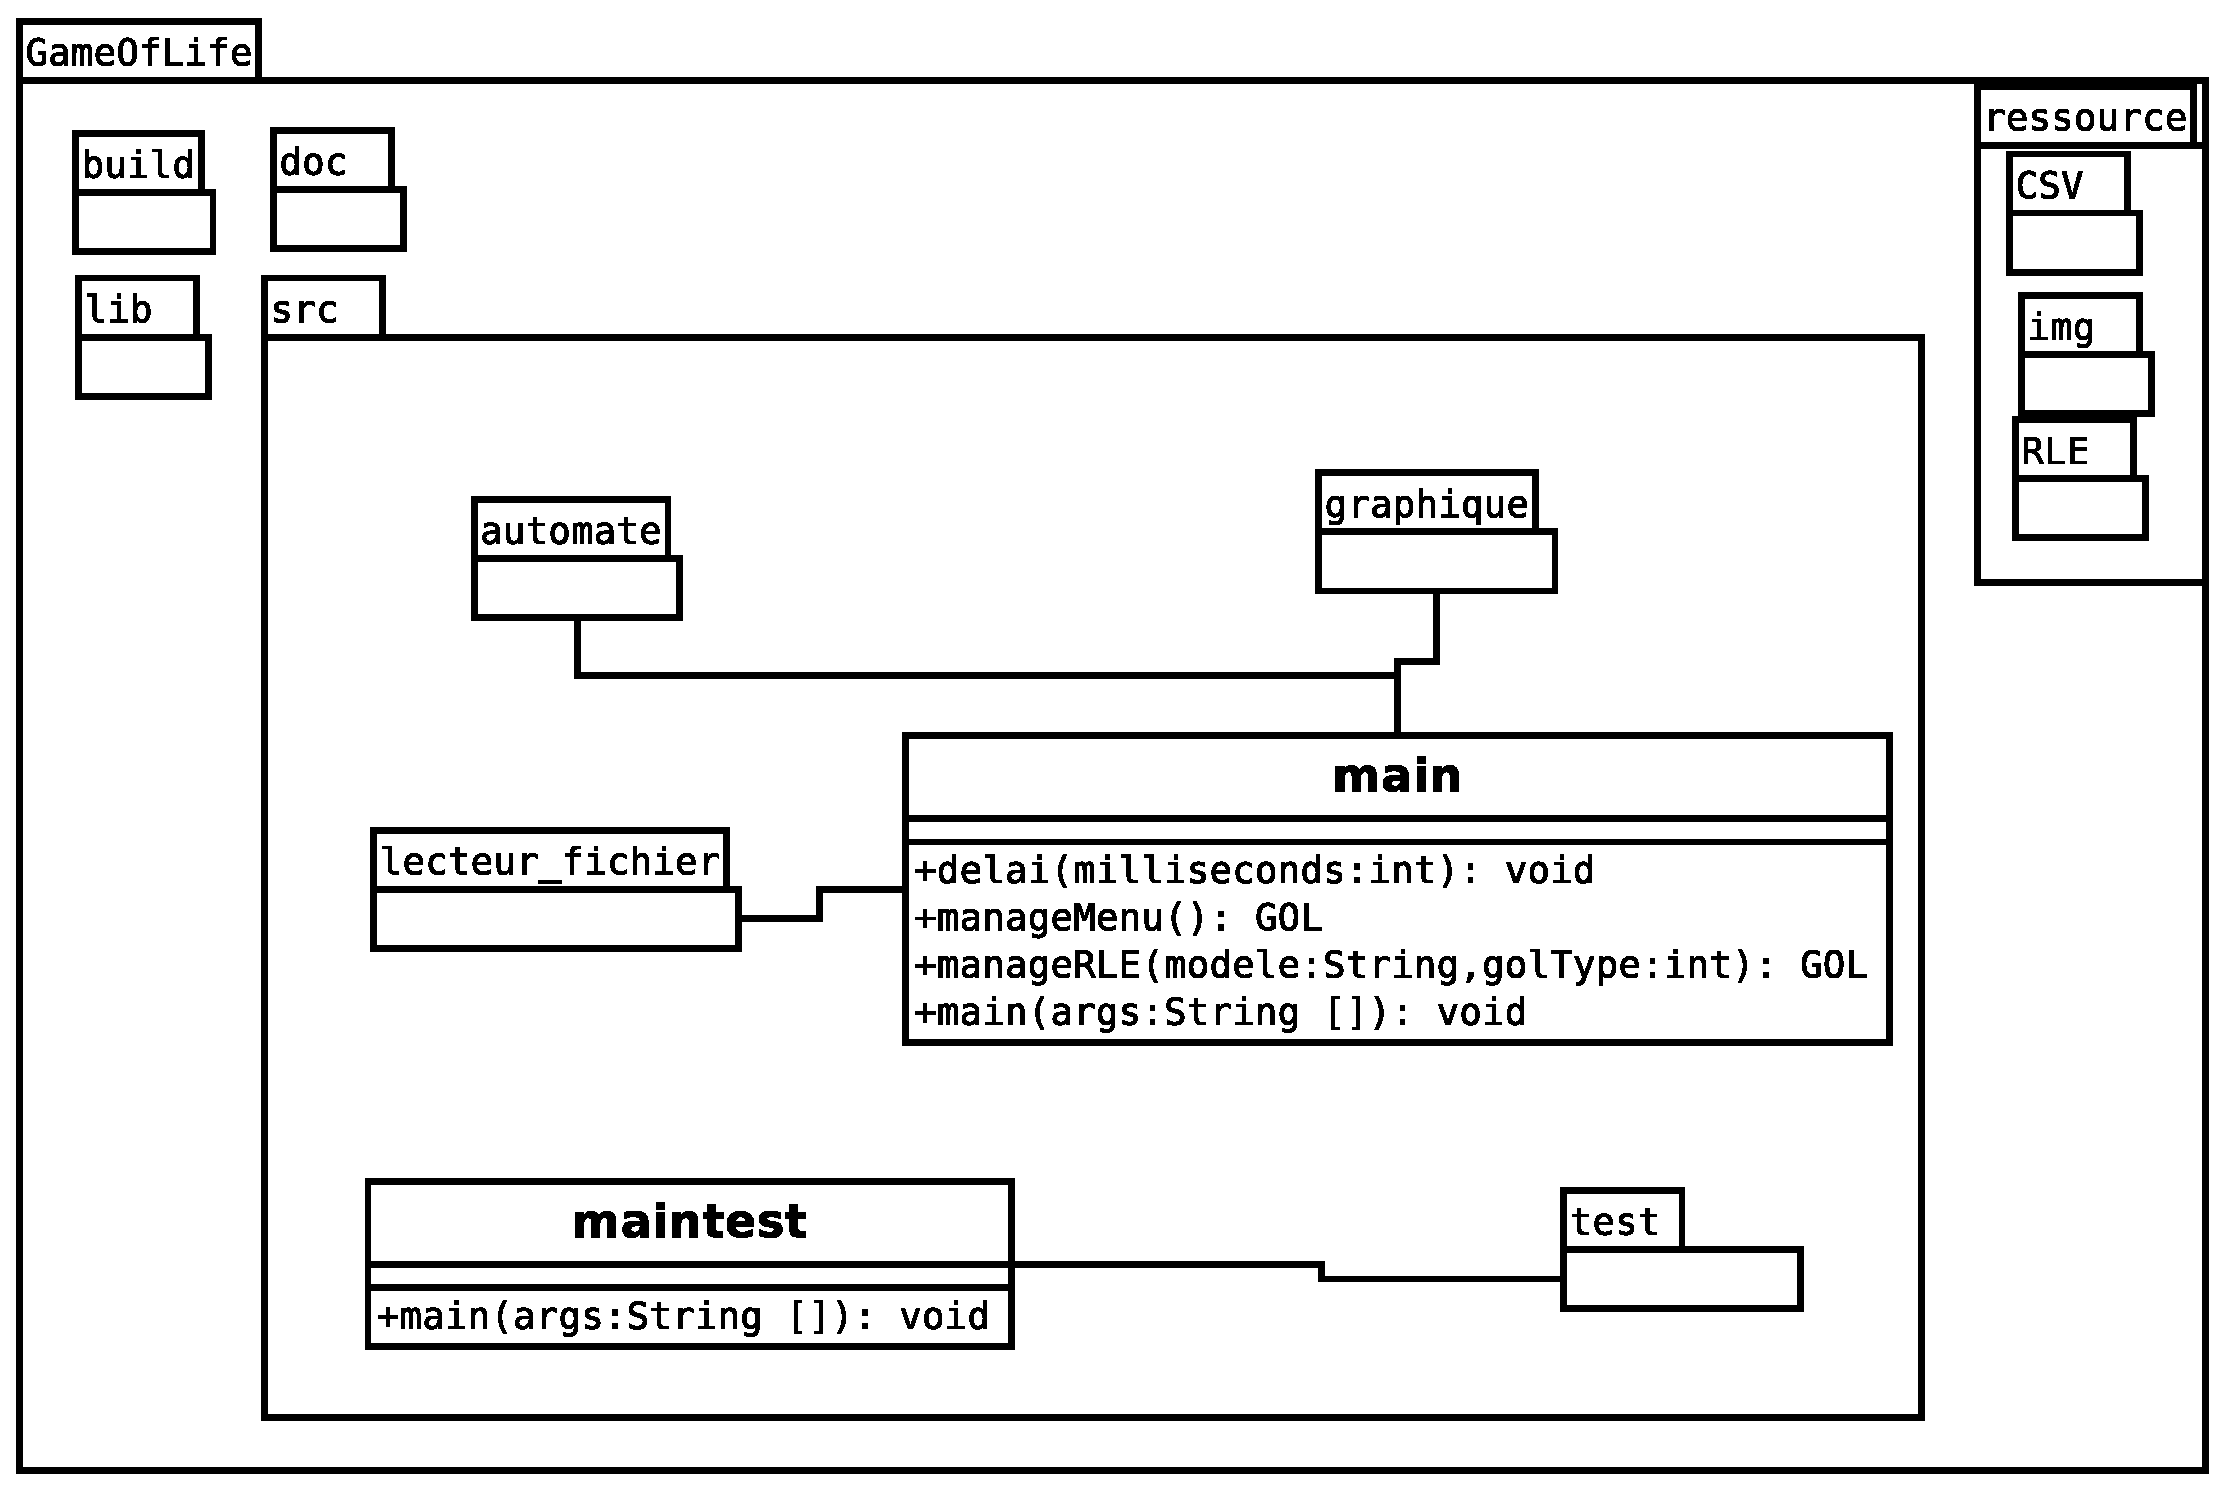
\includegraphics[scale=0.35]{images/Diagramme/Projet.eps}
\caption{\label{fig:GameOfLife}Illustration du package GameOfLife}
\end{figure}

\par Dans le package src nous avons différents package ainsi que les deux classes main : \begin{itemize}
    \item La classe \textbf{main} qui lance le jeu de la vie.
    \item La classe \textbf{maintest} qui lance tout les tests présents dans le package test et affiche la réussite ou l'échec de chacun.
\end{itemize}
\par Parmi les différents package nous avons les quatre suivants : \begin{itemize}
    \item Le package \textbf{automate}
    \item Le package \textbf{graphique}
    \item Le package \textbf{lecteur fichier}
    \item Le package \textbf{test}
\end{itemize}
\subsection{Package Automate}

\par Le package \textbf{automate} va initialiser les différentes versions du jeu de la vie ou de l'automate cellulaire. Il est composé de deux sous-package : \begin{itemize}
    \item Le package \textbf{gridlife} initialisant les différentes versions d'automates cellulaires sur une grille.
    \item Le package \textbf{hashlife} initialisant le jeu de la vie sur un ensemble de quadtree.
\end{itemize}

\par Ce package compte aussi deux classes abstraites et une interface qui initialise les méthodes communes au deux package.
La classe abstraite \textbf{GOL} généralise les variables communes et les fonction utilisées dans les classes qui l'héritent (\textbf{GOLqTree}, \textbf{GOLGrille}), cette classe va être utilisée dans l'interface et le main afin de pouvoir changer rapidement d'instance de \textbf{GOL} et initialiser les modèles RLE. \\
La classe abstraite \textbf{Decode} va servir a décoder les règles du jeu de la vie ou de l'automate cellulaire. Elle contient les règles ainsi qu'une méthode abstraite qui doit vérifier si les règles sont valides ainsi qu'un accesseur. Cette classe sera hérité par une classe pour chaque instance différente de \textbf{GOL} : 
\begin{itemize}
    \item la classe \textbf{DecodeqTree} dans le package hashlife qui va décoder les règles de format standard du jeu de la vie (B.../S...) exemple : Conway's Life (premier jeu de la vie) a pour règles B3/S23 .
    \item la classe \textbf{DecodeGrilleLifeLike} dans le package gridlife qui va décoder les règles de format (././././././././././././././././) prenant 15 chiffres entier entre 0 et 15 (inclus) qui est utilisé pour les algorithmes neuraux.
    \item la classe \textbf{DecodeGrilleMargolus} dans le package gridlife qui va décoder les règles de format (././././././././) prenant 8 chiffres entre 0 et 1 qui est utilisé pour les voisinages de Margolus.
\end{itemize}
\begin{figure}[htp]
\centering
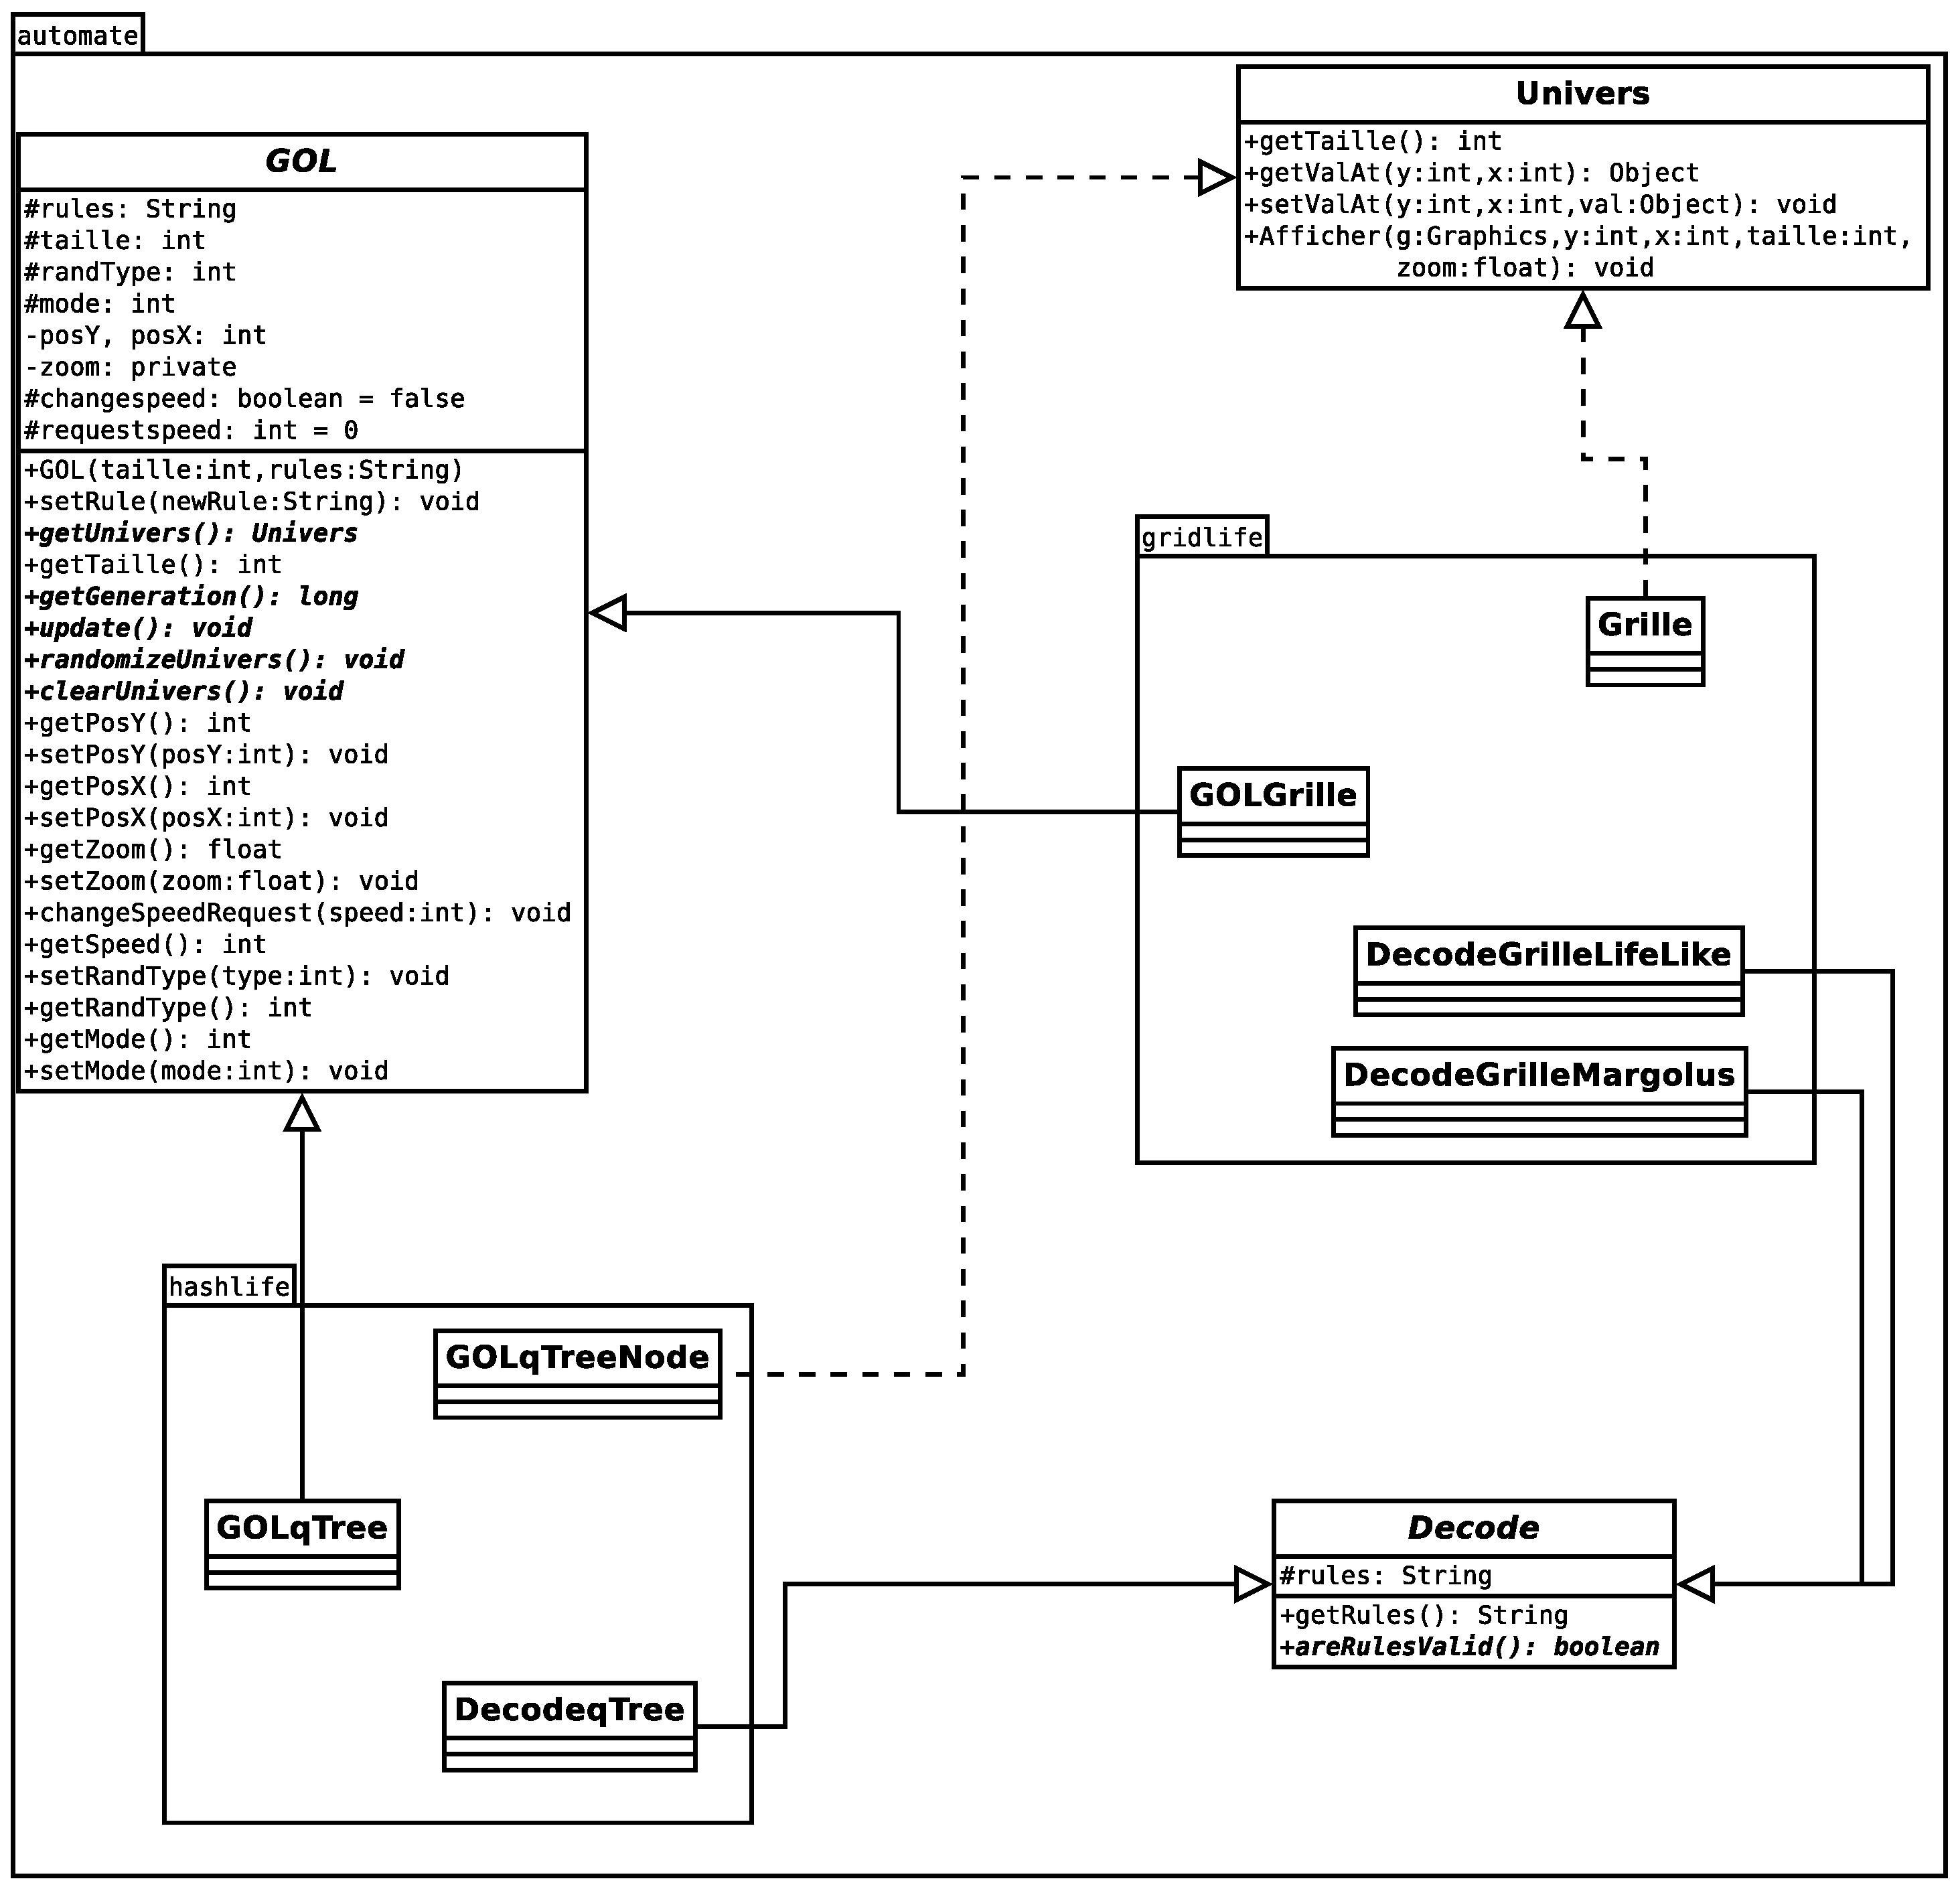
\includegraphics[scale=0.25]{images/Diagramme/package_automate.eps}
\caption{\label{fig:Automate}Illustration du package automate}
\end{figure}
\par L'interface Univers va être implémentée par les "supports" du jeu de la vie ou des automates cellulaires. La classe \textbf{Grille} dans le package gridlife et la classe \textbf{GOLqTreeNode} dans le package hashlife. Cette interface va initialisé les accesseurs et modificateurs de valeur à une certaine coordonnée ainsi qu'une méthode permettant l'affichage sur un Graphics.
\subsubsection{package gridlife}
\par Le package gridlife va représenter les automates cellulaires sur grille. Il est composé des différentes classes héritant du package automate : \begin{itemize}
    \item la classe \textbf{Grille}
    \item la classe \textbf{GOLGrille}
    \item la classe \textbf{DecodeGrilleLifeLike}
    \item la classe \textbf{DecodeGrilleMargolus}
\end{itemize}

\begin{figure}[htp]
\centering
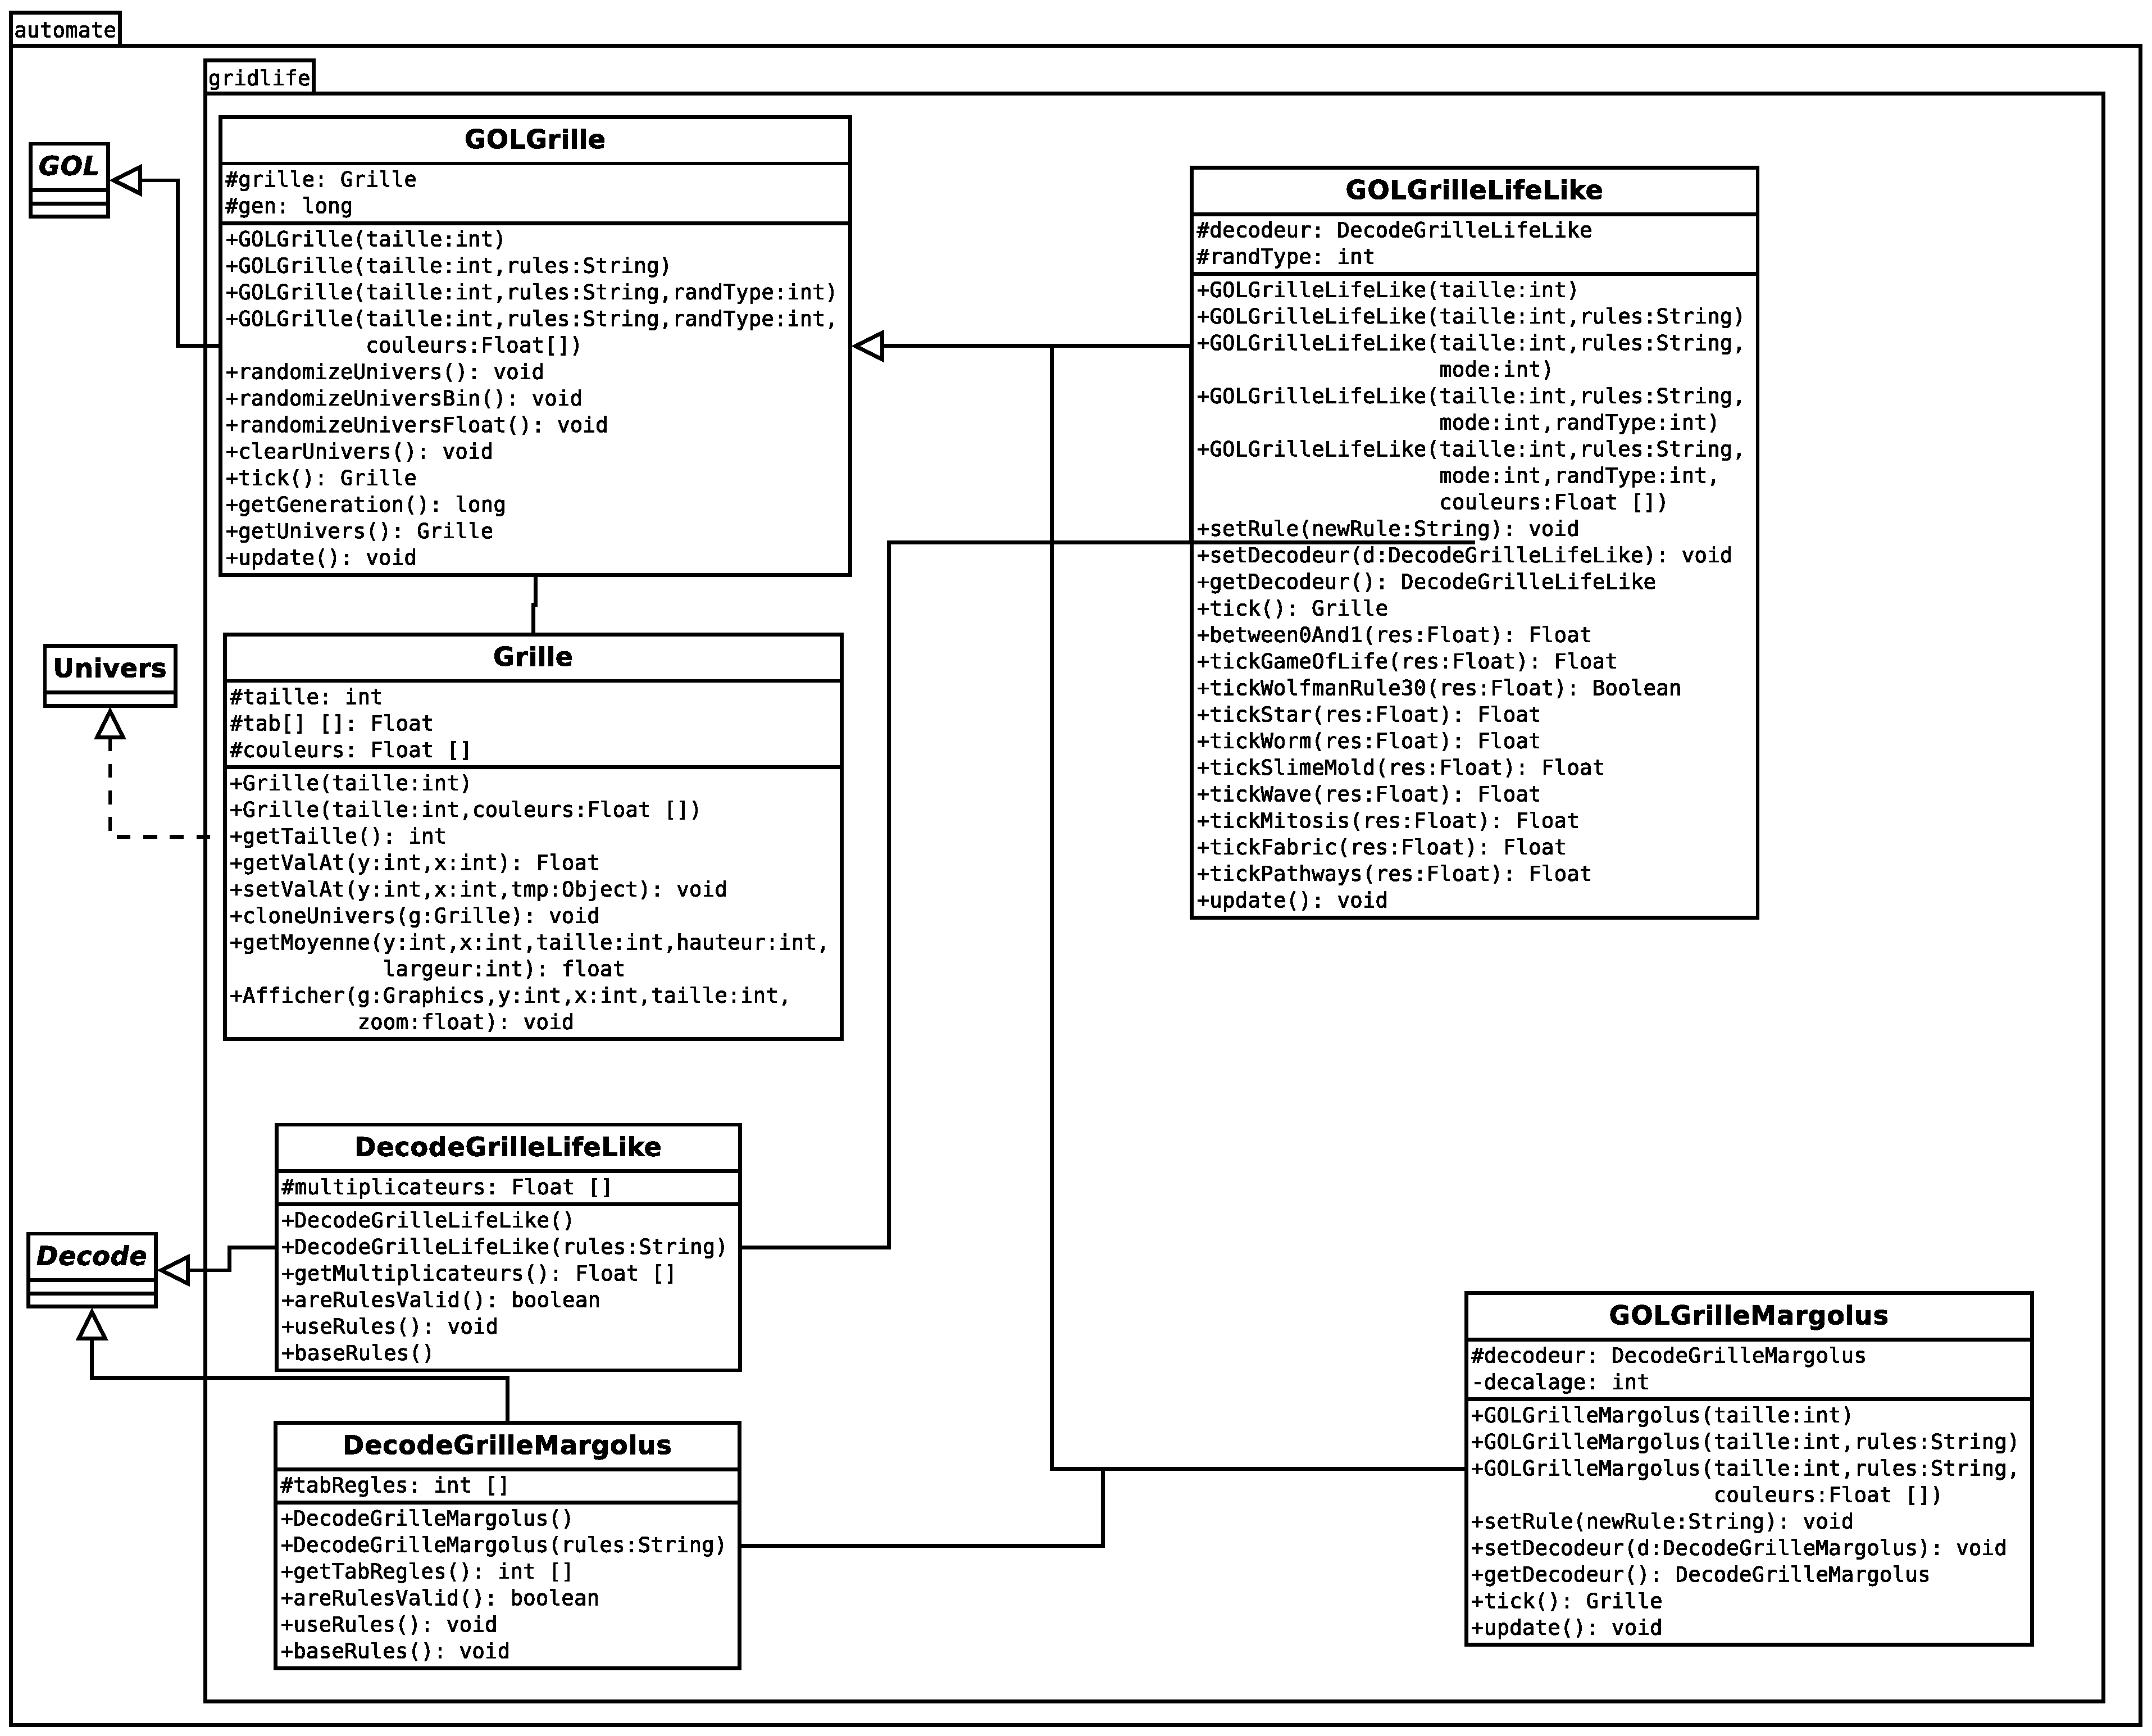
\includegraphics[scale=0.25]{images/Diagramme/package_automate_gridlife.eps}
\caption{\label{fig:Automate/gridlife}Illustration du package automate/gridlife}
\end{figure}
\par Il contient aussi les classes \textbf{GOLGrilleLifeLike} et \textbf{GOLGrilleMargolus} héritant de \textbf{GOLGrille} qui définissent et lancent les différentes versions des automates cellulaires et utilisent les différents décodeur respectivement les algorithmes neuraux et les voisinages de Margolus.
\subsubsection{package hashlife}
Le package hashlife regroupent toutes les classes permettant d'initialiser le jeu de la vie avec des quadtrees. Il est composé des différentes classes héritant du package automate :\begin{itemize}
    \item La classe \textbf{GOLqTreeNode}
    \item La classe \textbf{GOLqTree}
    \item La classe \textbf{DecodeQtree}
\end{itemize}
\begin{figure}[htp]
\centering
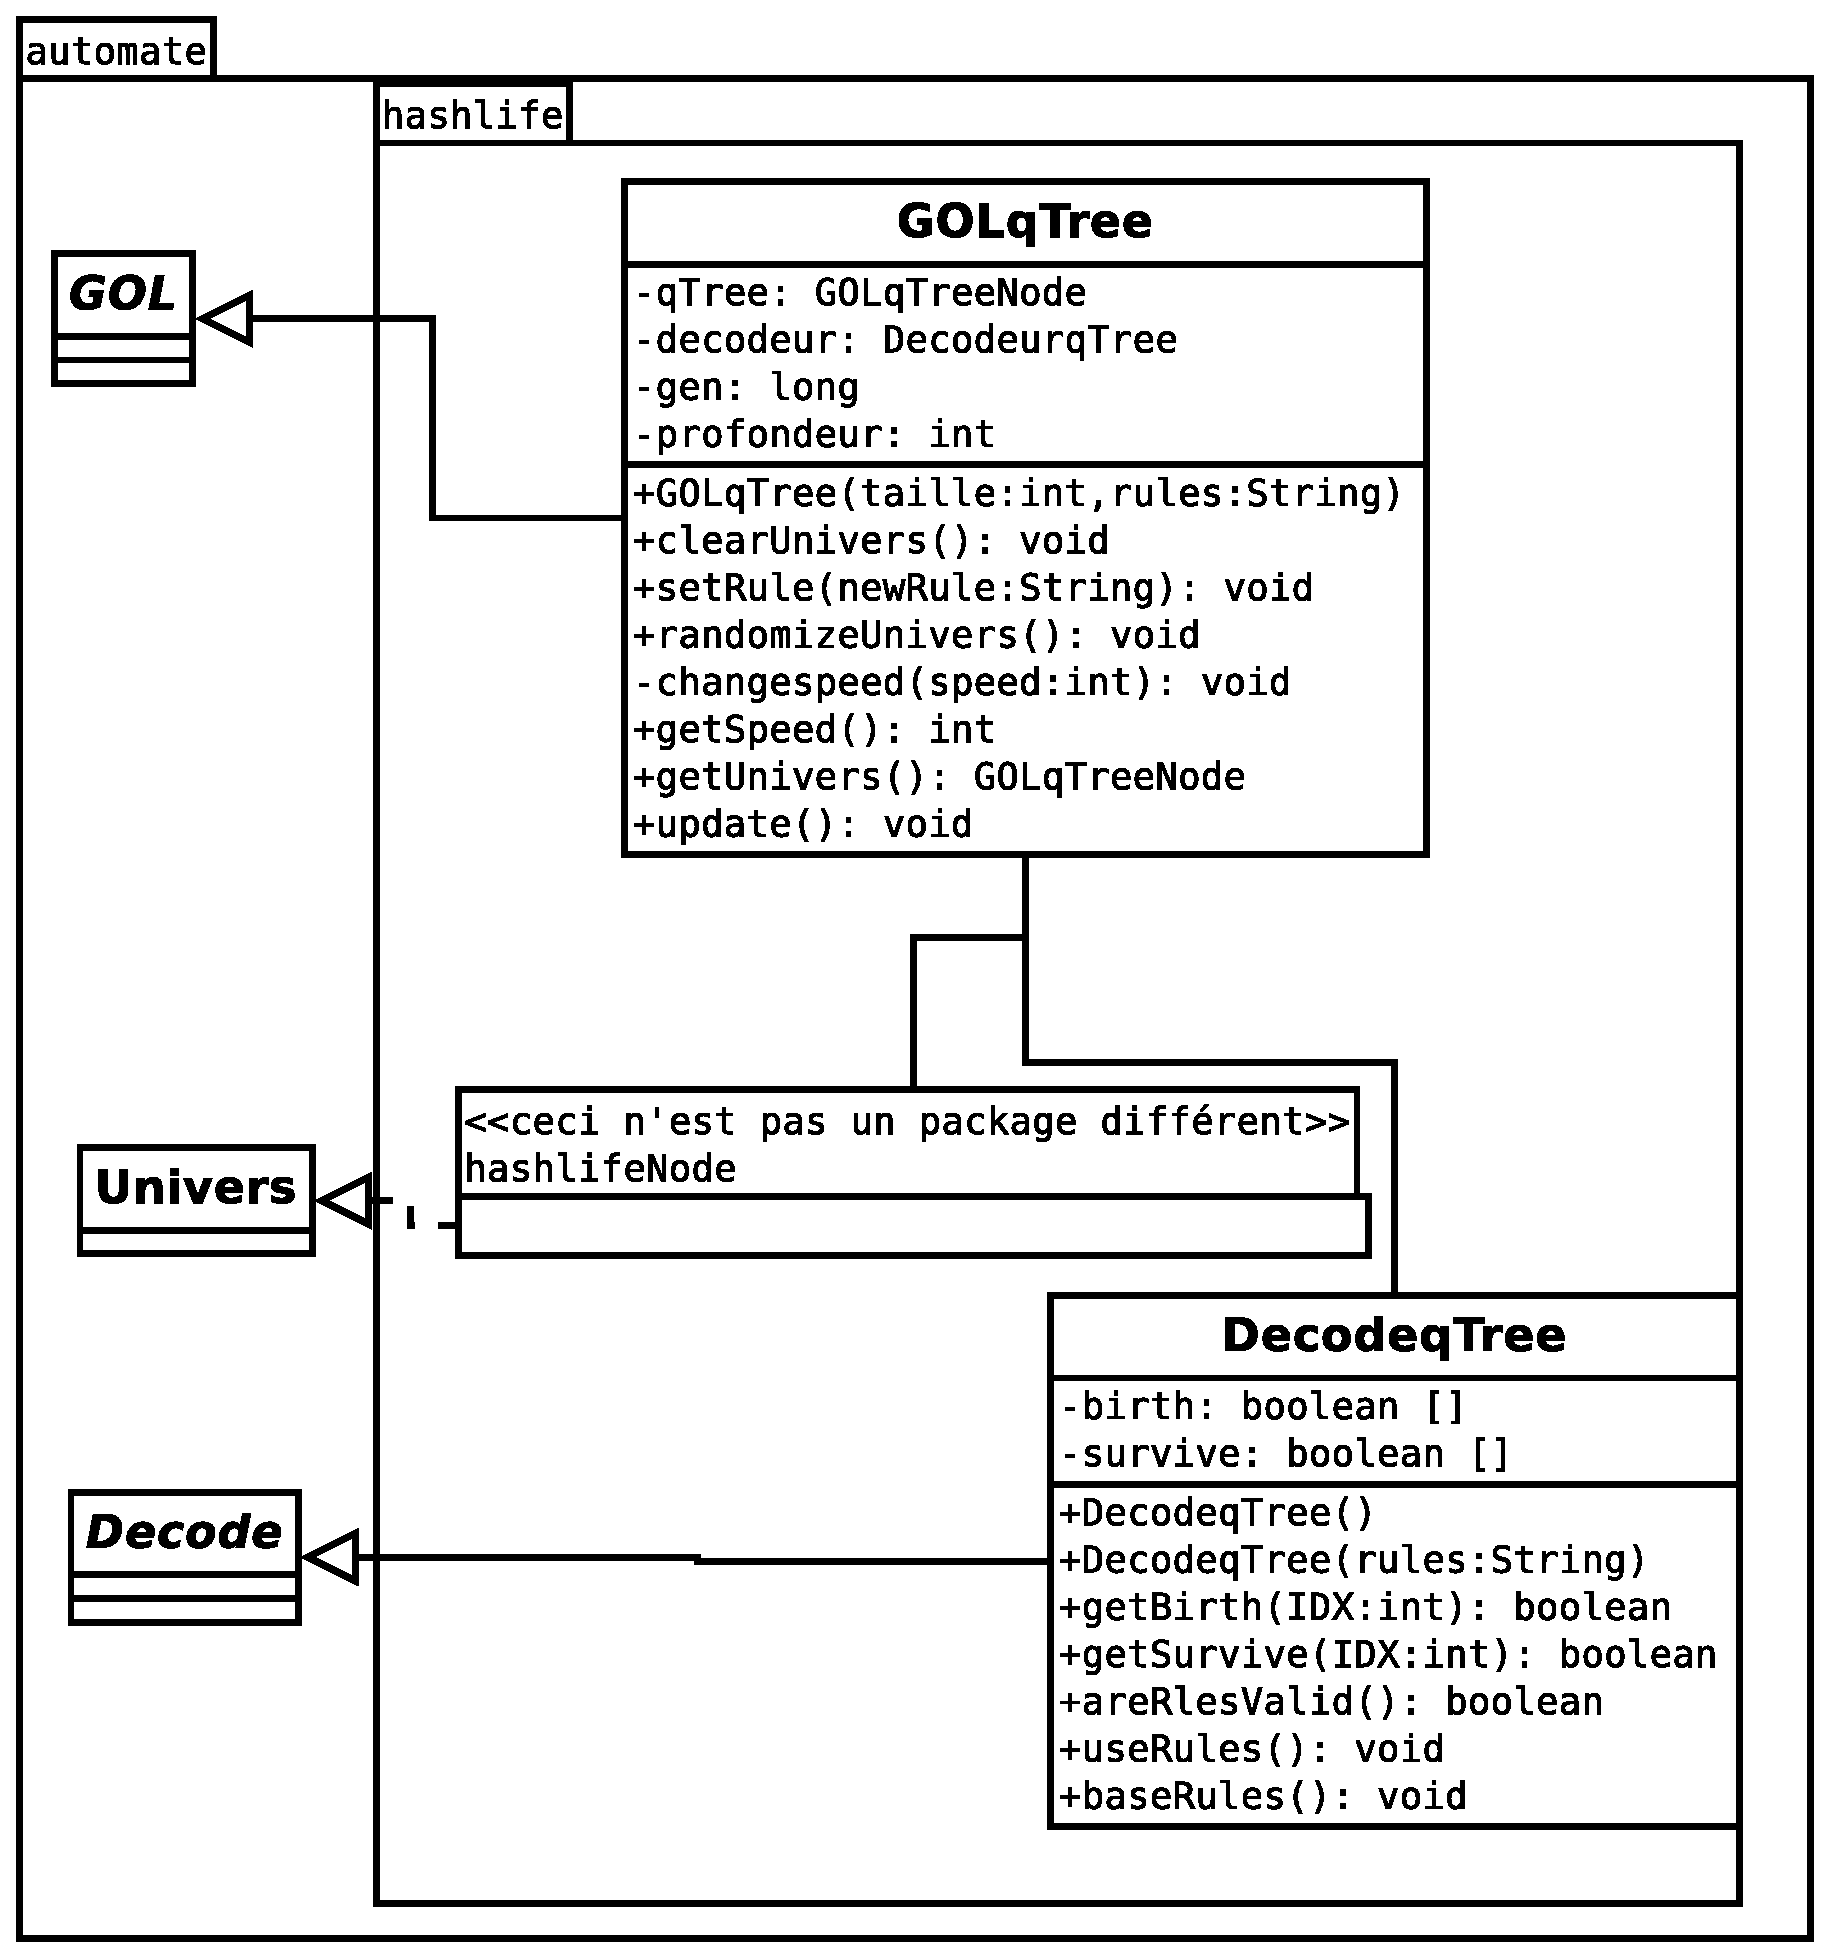
\includegraphics[scale=0.35]{images/Diagramme/package_automate_hashlife.eps}
\caption{\label{fig:Automate/hashlife}illustration du package automate/hashlife}
\end{figure}
\par Il contient également les classes permettant de placer le quadtree dans une hashMap (\textbf{CanonicalizedqTree}), une autre classe implémentant Almost-Hashlife (\textbf{MemoizedqTree}) ainsi qu'une classe implémentant hashlife (\textbf{HashlifeqTree}).
\begin{figure}[htp]
\centering
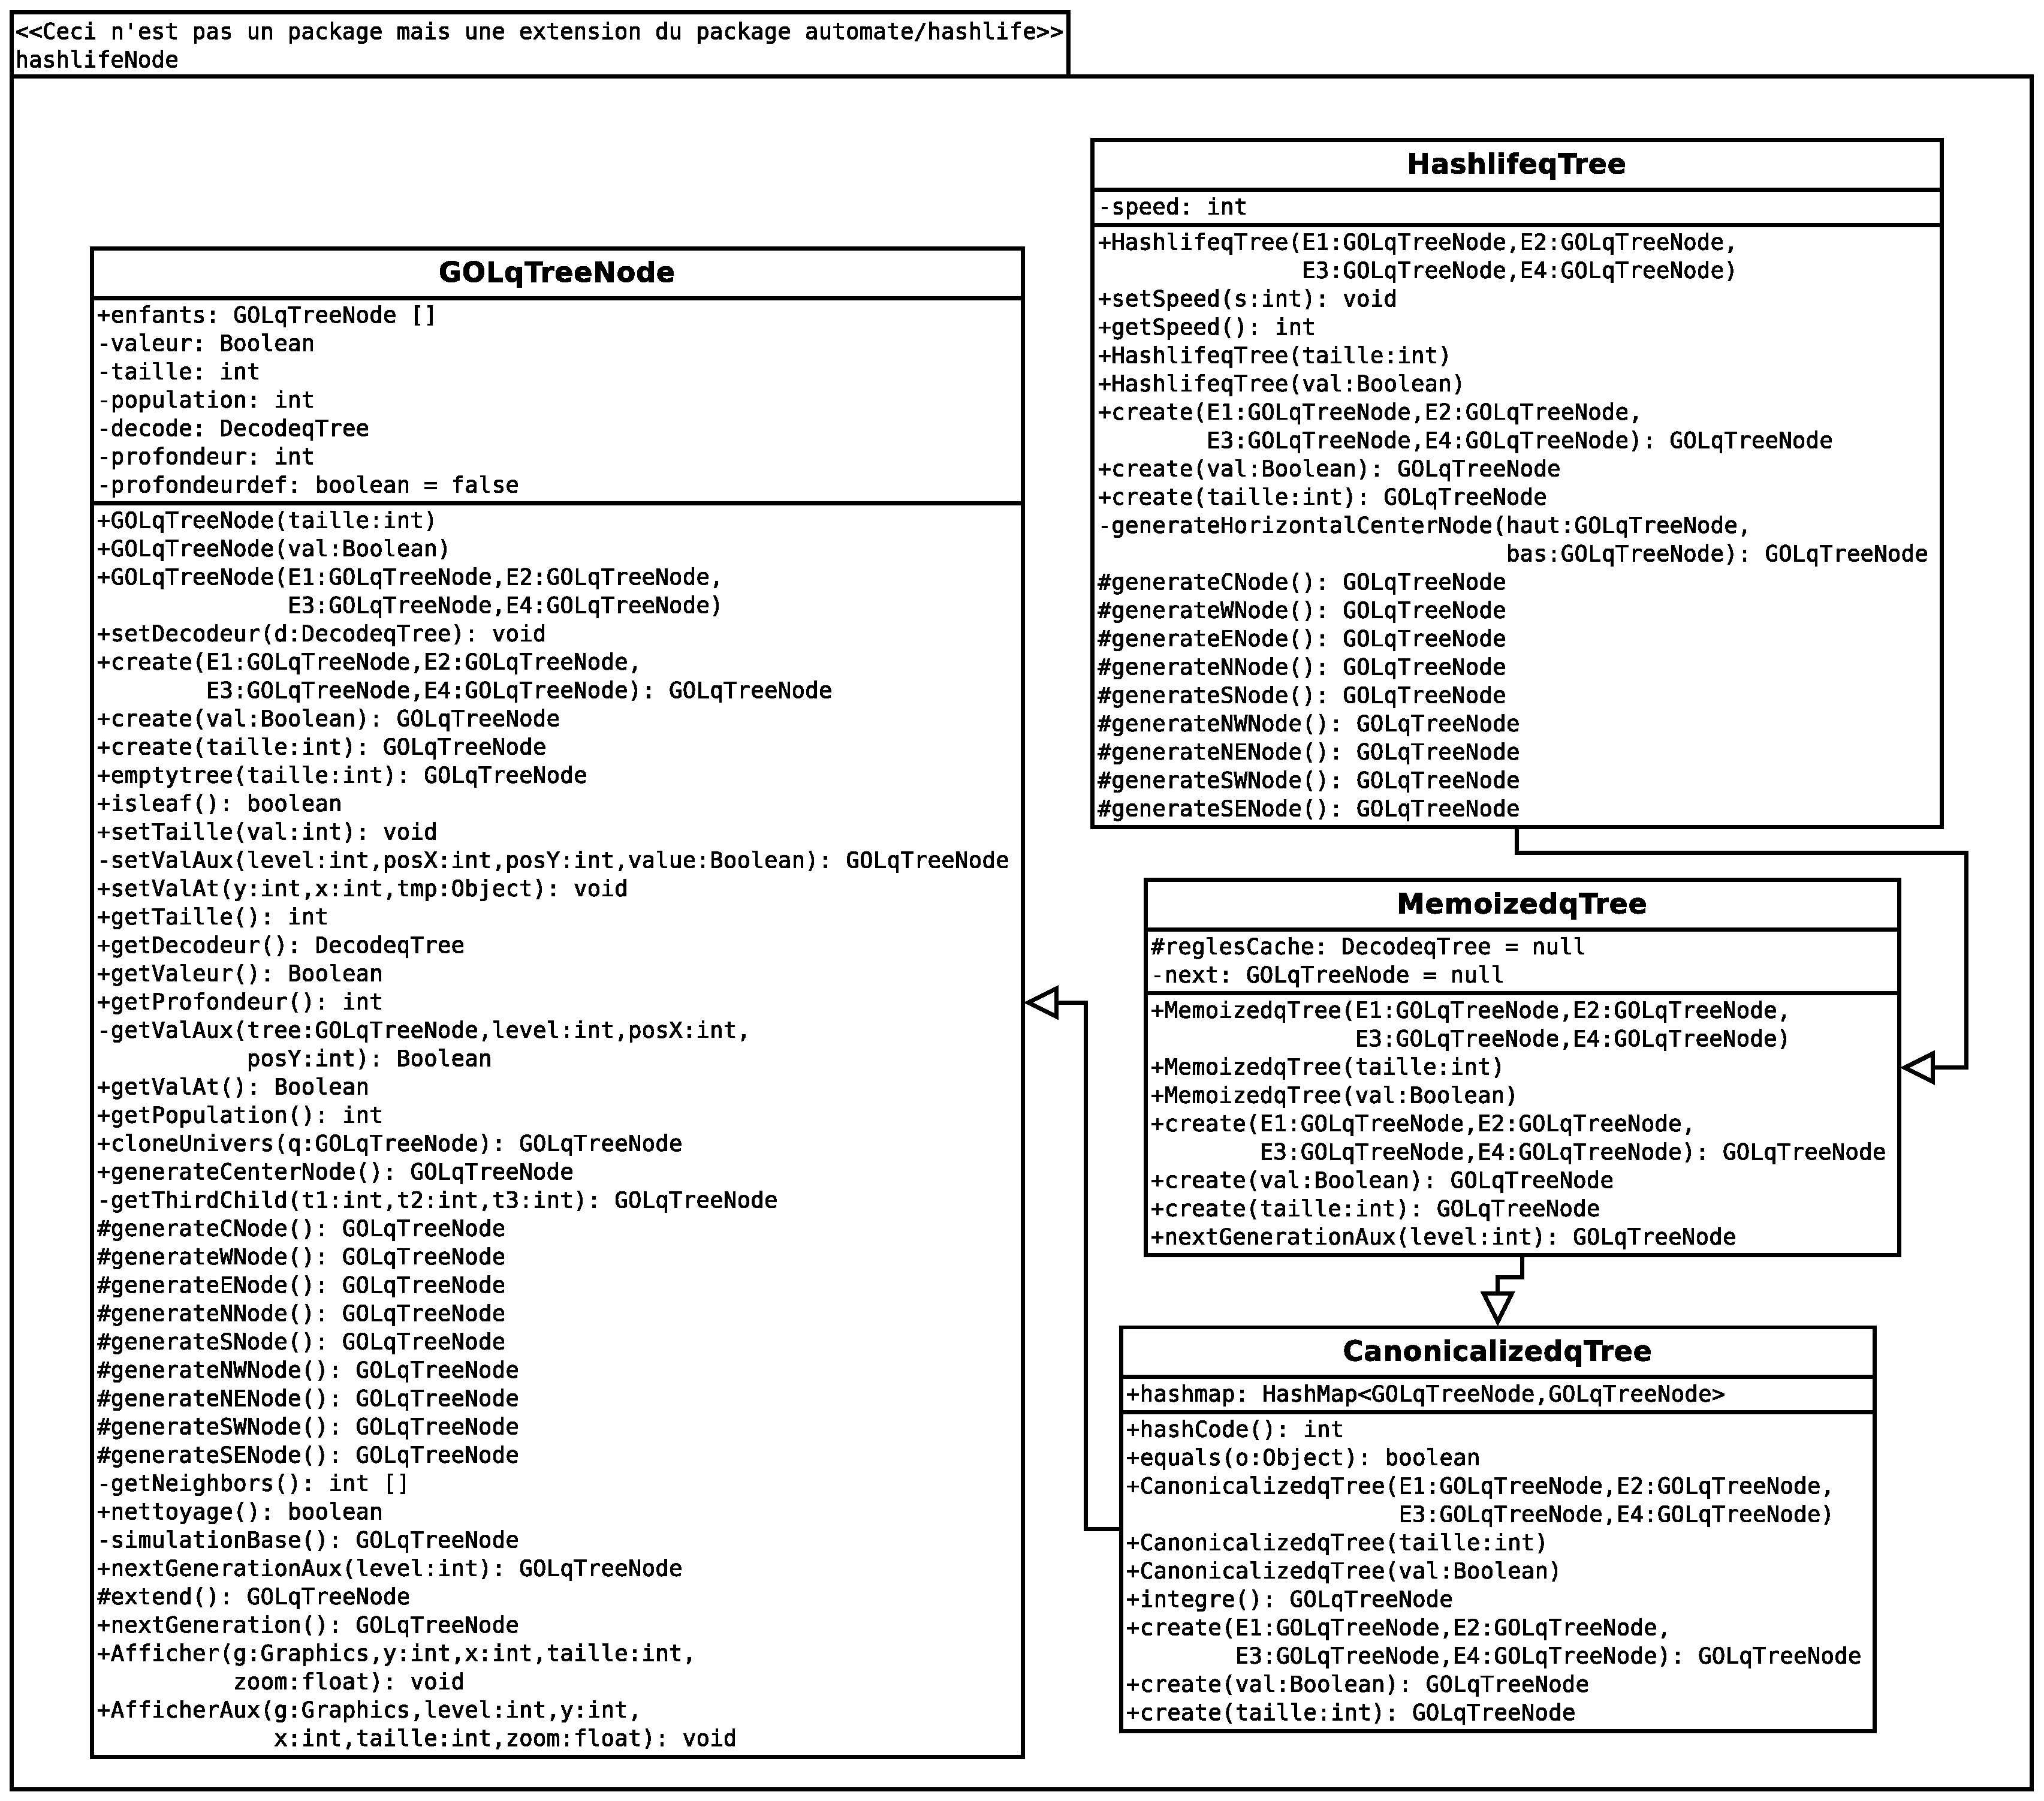
\includegraphics[scale=0.22]{images/Diagramme/package_automate_hashlifeNode.eps}
\caption{\label{fig:Automate/hashlifeNode}Illustration de la partie hashlifeNode du diagramme précédent}
\end{figure}
\subsection{Package Graphique}
\par Le package graphique regroupe tout ce qui a un rapport avec l'interface comme les interaction entre le clavier et l'interface via la classe \textbf{Clavier} qui implémente l'interface KeyListener ou encore l'interface elle même (\textbf{InterfaceGameOfLife}) avec ces différents composants (\textbf{AffichagePrincipal}, \textbf{Menu}). 
\begin{figure}[htp]
\centering
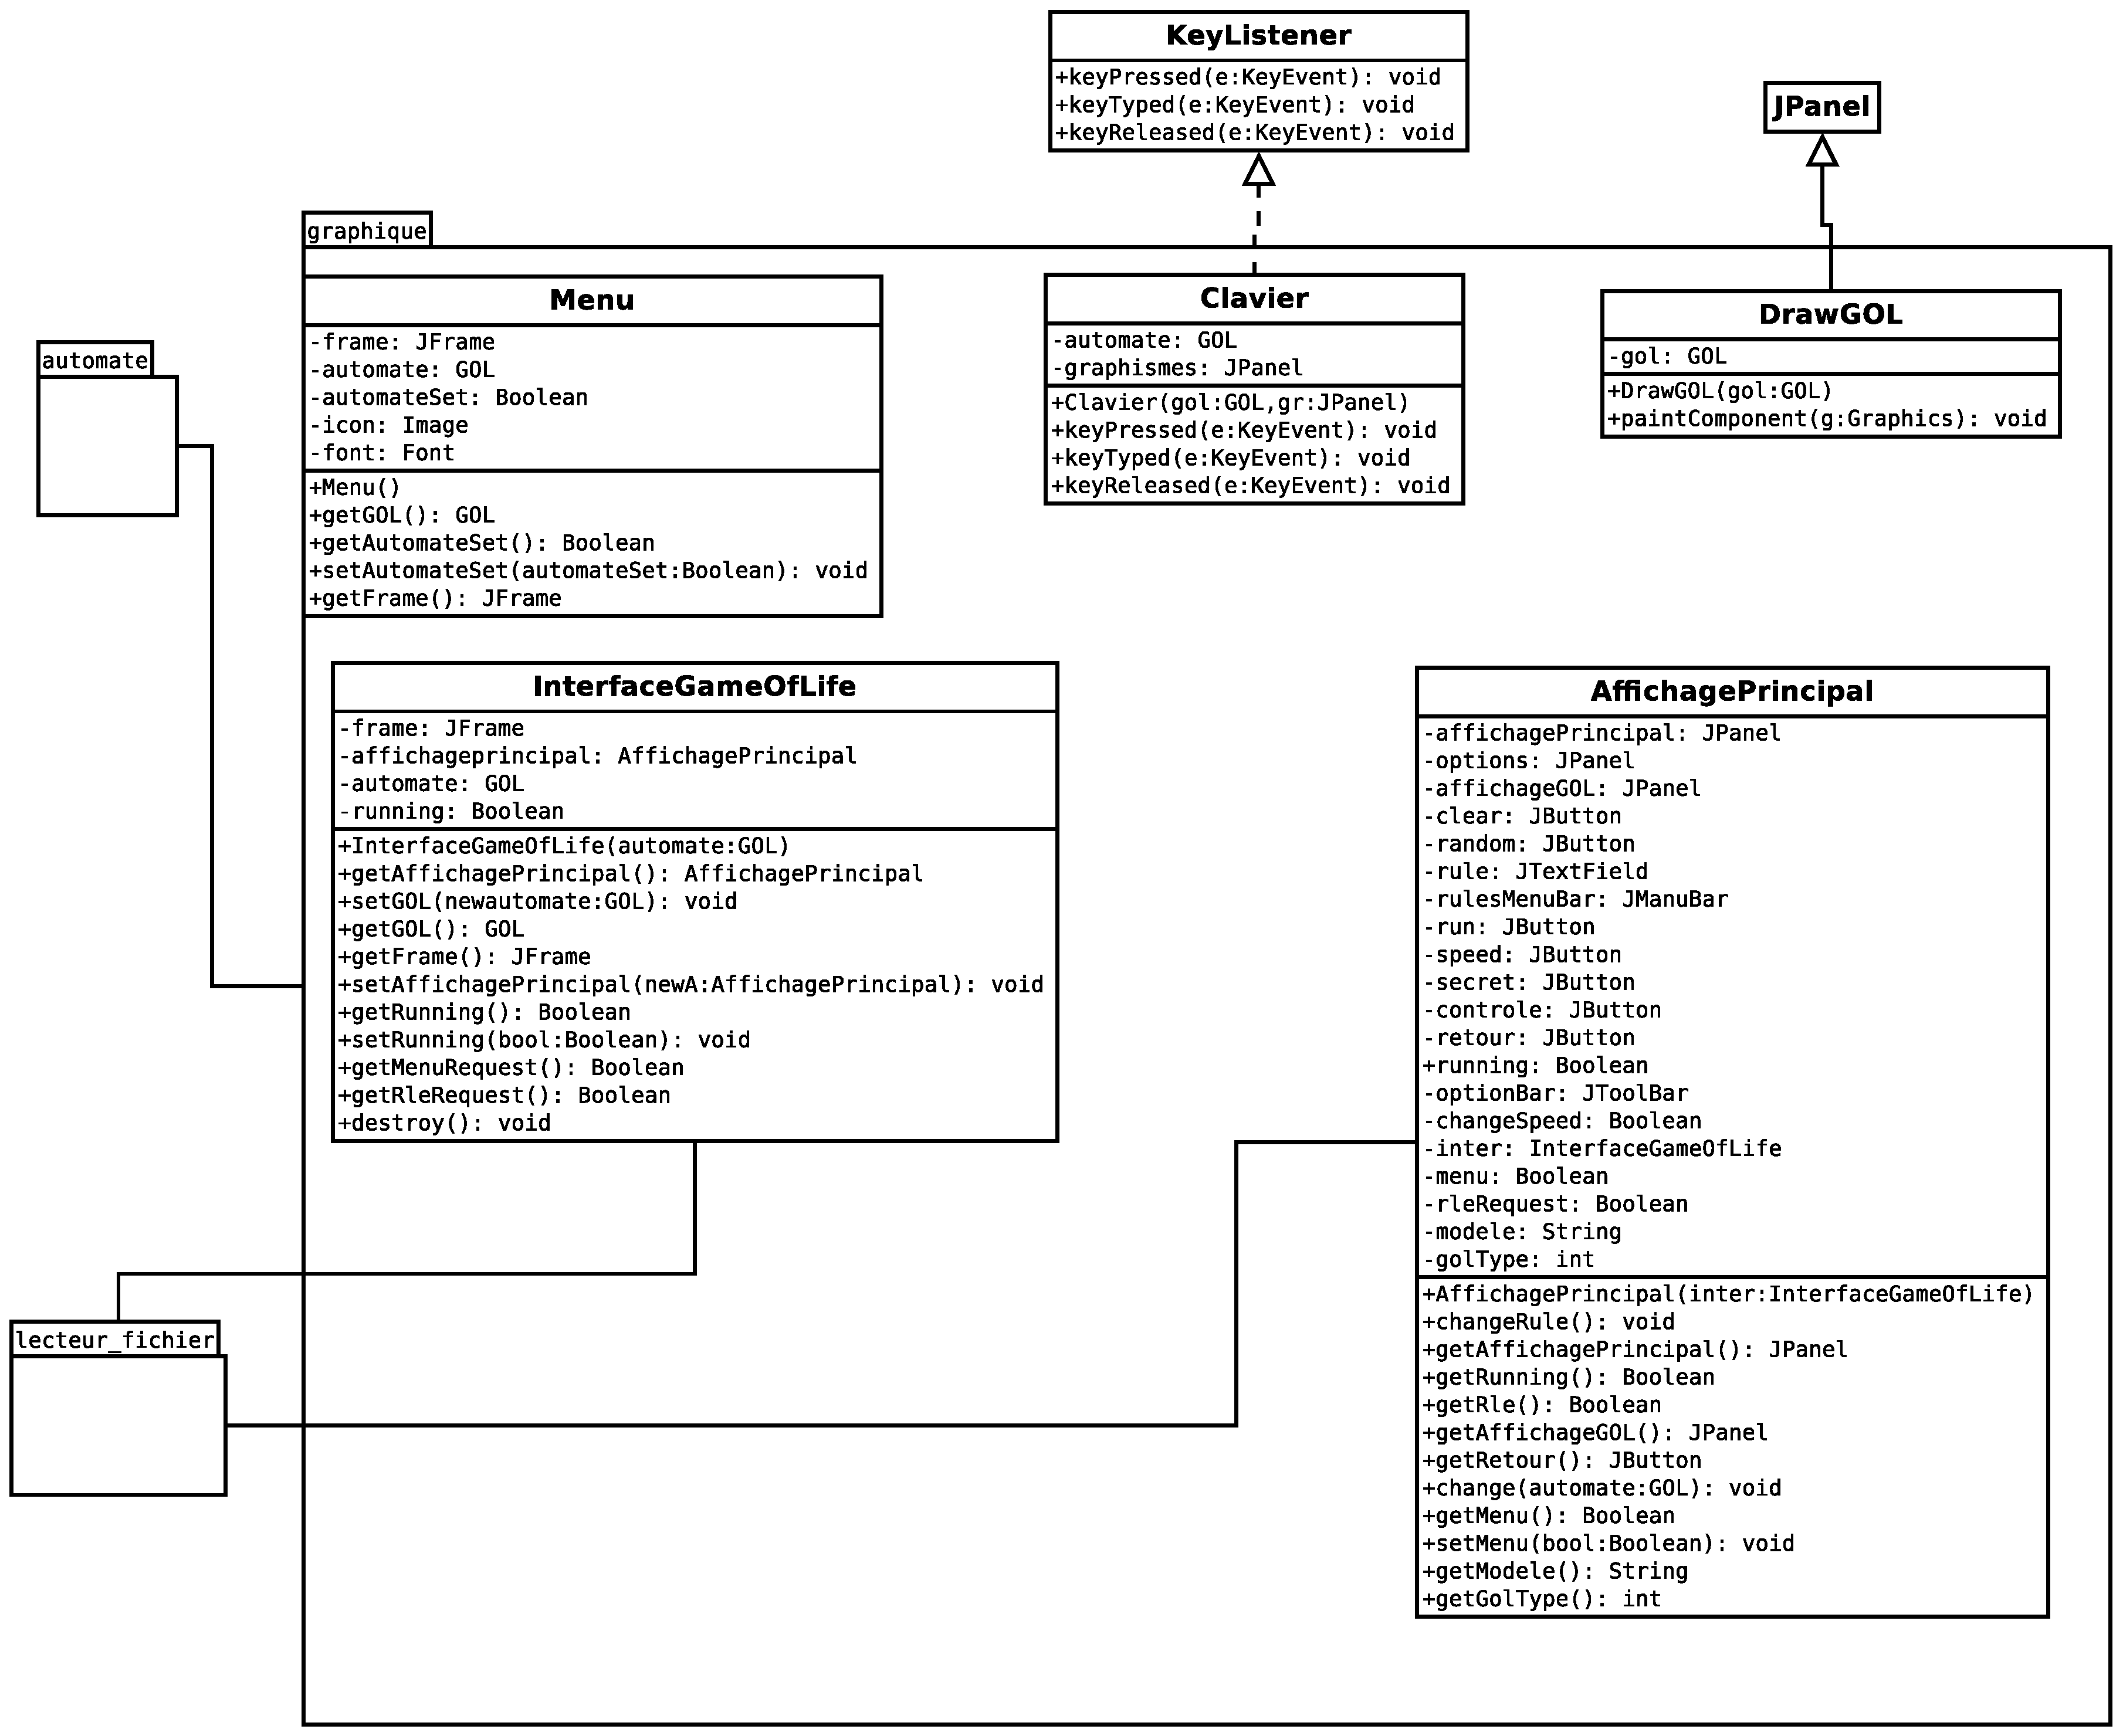
\includegraphics[scale=0.22]{images/Diagramme/package_graphique.eps}
\caption{\label{fig:Graphique}Illustration du package graphique}
\end{figure}
\subsection{Package Lecteur fichier}
\par Le package lecteur fichier contient les classes permettant la lecture des différents fichiers en ressources.\\
La classe \textbf{Lecture CSV} permet de lire un fichier CSV et renvoie les informations dans une liste de tableaux de chaînes de caractères (un tableau de chaînes de caractères représentent une ligne du fichier CSV). Cette classe a aussi d'autres méthodes permettant de rechercher le code (ou mode ou type d'univers aléatoire (uniquement pour les instance de \textbf{GOLGrilleLifeLike}))  du jeu de la vie ou de l'automate cellulaire grâce aux noms (ou au code) du jeu de la vie ou de l'automate cellulaire.\\
La classe \textbf{LecteurRLE} permet de charger un modèle RLE sur une instance de \textbf{GOL} après l'avoir récupéré et décodé de l'archive.
\\
Ce package va être réutilisé par les classes du package graphique ainsi que par le main.
\begin{figure}[htp]
\centering
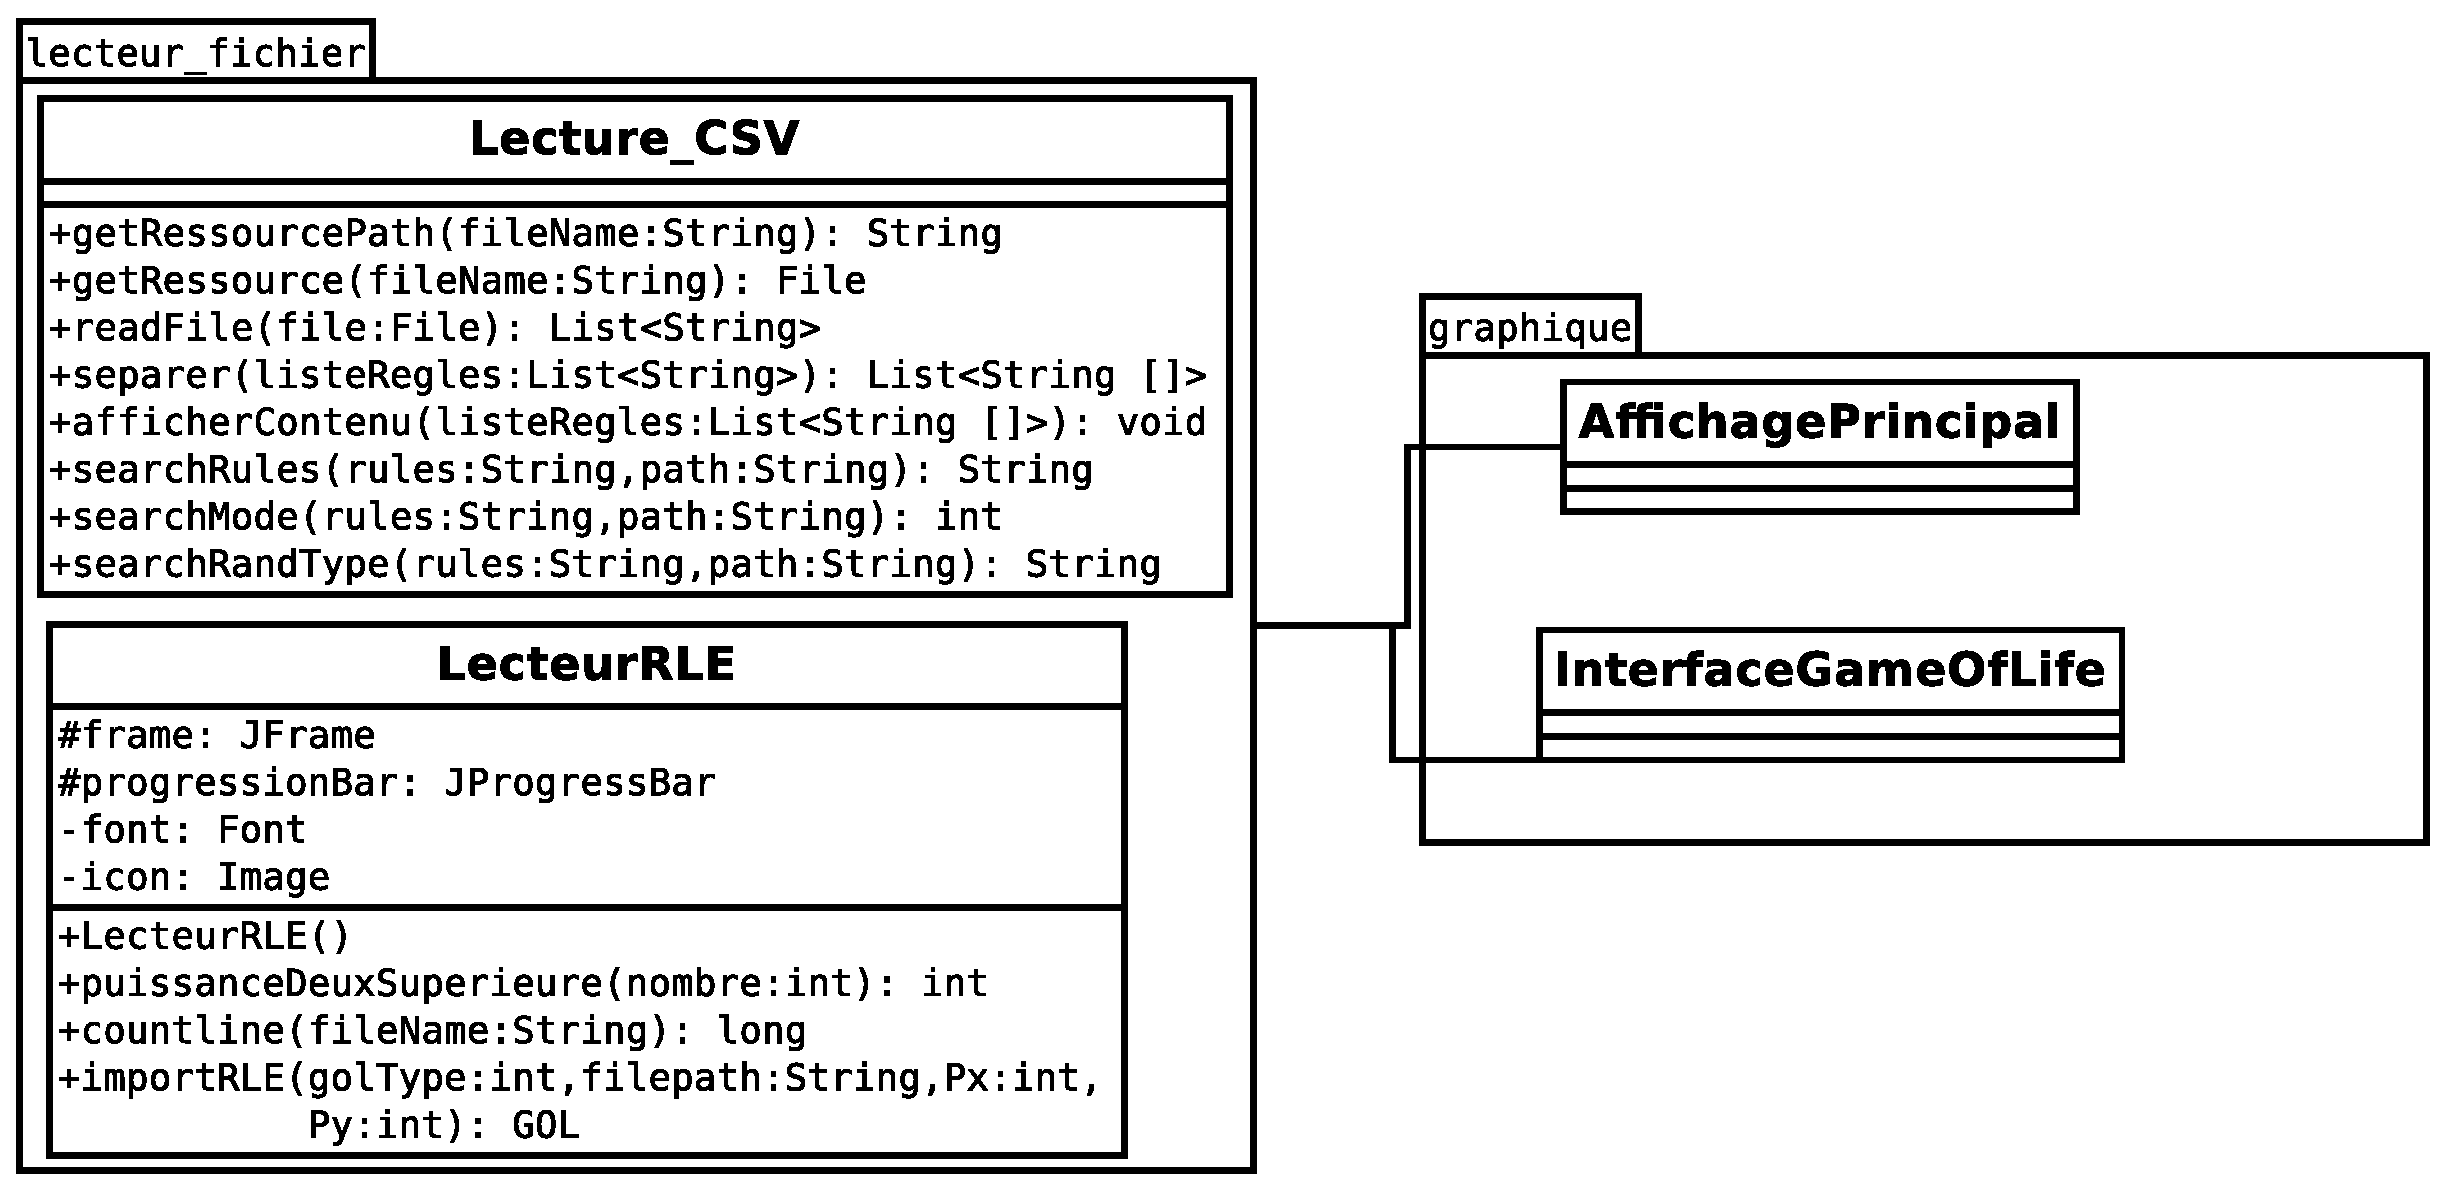
\includegraphics[scale=0.35]{images/Diagramme/package_lecteur_fichier.eps}
\caption{\label{fig:Lecteur_fichier}illustration du package lecteur fichier}
\end{figure}
\subsection{Package Test}
Ce package contient tout les test unitaires du projet permettant de savoir la validité des méthodes utilisées dans les différentes classes des package automate et lecteur fichier.